% Generated by experiments/exp2_thesis/make_assets.py -- do not edit by hand.
\begin{figure}[tbp]
  \centering
  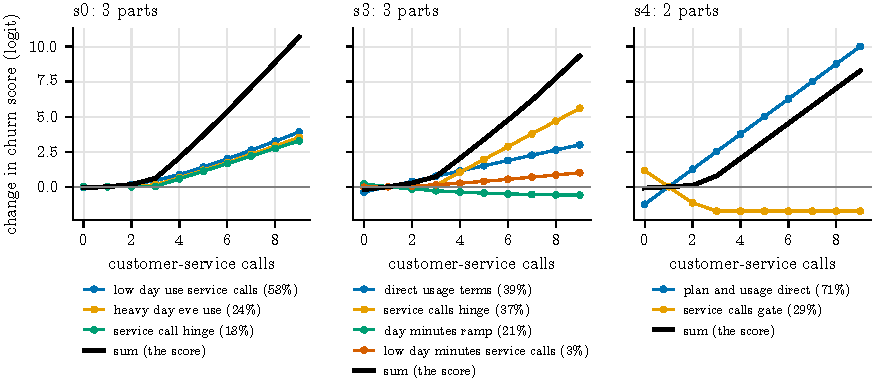
\includegraphics[width=\textwidth]{figures/exp2/exp2-churn-calls-parts}
  \caption{Churn: one signal, three realisations. The score's response to customer-service calls (mean over training customers, relative to 1 call) is split into the explanation parts that carry it; the parts sum exactly to the score's response (black). Seed 0 spreads the threshold over three parts, seed 3 builds it from a direct slope, a threshold hinge and a day-usage ramp, and in seed 4 a gate cancels the direct slope at low call counts (the two parts point in opposite directions; cancellation ratio 0.19). Legend: each part's share of the response's variance.}
  \label{fig:exp2-churn-calls-parts}
\end{figure}
